\documentclass[11pt]{article}

% ---- Geometry & typography ---------------------------------------------------
\usepackage[a4paper,margin=0.95in]{geometry}
\usepackage{microtype}
\usepackage{lmodern}
\usepackage[T1]{fontenc}
\usepackage[utf8]{inputenc}
\usepackage{titlesec}
\usepackage{enumitem}
\setlist{nosep, leftmargin=*}
\titlespacing*{\section}{0pt}{1.4ex}{0.6ex}
\titlespacing*{\subsection}{0pt}{1.0ex}{0.4ex}
\titleformat{\section}{\large\bfseries}{\thesection}{0.5em}{}
\titleformat{\subsection}{\normalsize\bfseries}{\thesubsection}{0.5em}{}

% ---- Math --------------------------------------------------------------------
\usepackage{amsmath,amssymb,amsthm,bm}
\usepackage{mathtools}
\DeclarePairedDelimiter{\norm}{\lVert}{\rVert}
\DeclareMathOperator*{\argmin}{arg\,min}
\DeclareMathOperator*{\argmax}{arg\,max}
\DeclareMathOperator{\rank}{rank}
\DeclareMathOperator{\spark}{spark}
\DeclareMathOperator{\supp}{supp}
\DeclareMathOperator{\STFT}{STFT}
\DeclareMathOperator{\sgn}{sgn}
\newcommand{\R}{\mathbb{R}}
\newcommand{\E}{\mathbb{E}}
\newcommand{\D}{\bm{D}}
\newcommand{\xb}{\bm{x}}
\newcommand{\yb}{\bm{y}}
\newcommand{\alphab}{\bm{\alpha}}
\newcommand{\Mb}{\bm{M}}

% ---- Floats, tables, links ---------------------------------------------------
\usepackage{graphicx}
\usepackage{booktabs}
\usepackage{caption}
\captionsetup{font=small, labelfont=bf, skip=4pt}
\usepackage[hidelinks]{hyperref}
\usepackage{xcolor}
\definecolor{mygreen}{HTML}{0B4F2F}
\usepackage{tcolorbox}
\tcbset{colback=mygreen!4, colframe=mygreen!50, boxrule=0.4pt, arc=2pt,
        left=4pt, right=4pt, top=2pt, bottom=2pt}

% ---- TikZ for the pipeline diagram ------------------------------------------
\usepackage{tikz}
\usetikzlibrary{positioning, arrows.meta, shapes.geometric, fit, backgrounds}

% ---- Bibliography (manual to avoid external .bib) ---------------------------
\usepackage{etoolbox}

\title{\vspace{-2.0em}\textbf{Sparse, Low-Rank, and Deep:\\
A Compressed-Sensing Framework for Music Source Separation}\\[0.4em]
\large ENGS 109 (Spring 2026) Final Project Proposal}
\author{Taka Khoo \\ \small Thayer School of Engineering, Dartmouth College \\
\small \texttt{takakhoo@gmail.com}}
\date{\vspace{-1em}\today}

\begin{document}
\maketitle
\vspace{-2em}

% ====================================================================
\begin{tcolorbox}
\textbf{Abstract.}\;
This is the third time I have studied audio under Peter Chin.  My
undergraduate honors thesis built a $1.08$-billion-parameter Token
U-Net for full-mix \emph{restoration} on EnCodec
tokens~\cite{khoo2025tokenunet}.  My MS thesis built MODULO/Mozart~AI,
a co-creative DAW whose stem-\emph{separation} stage is currently
outsourced to the ElevenLabs cloud API.  ENGS 109 gives me the
toolkit (compressed sensing, sparse coding, low-rank recovery,
deep sparsity) to attack the same separation problem from a third
direction with theoretical guarantees the deep-learning baselines
lack.  I propose a single spectrogram-domain pipeline that touches
five pillars of the course: Robust PCA harmonic--percussive
decomposition (L13), Non-negative Matrix Factorization with
class-conditional dictionaries (L15), K-SVD discriminative dictionary
learning with sparse-representation classification (L14, L8), a Deep
Sparse Coding Network mask predictor that adapts Chin's SparseNet
architecture to spectrogram regression (L16, never tried in this
regime), and Multiple-Measurement-Vector joint sparsity across stereo
channels (L12).  \textbf{Concrete novelty claim:} SparseNet has been
benchmarked only on image classification; this project is the first
adaptation of its composite-sparse-coding modules to a dense
regression task on audio spectrograms, evaluated head-to-head against
Demucs~v4 and the ElevenLabs baseline on MUSDB18-HQ.  A Day-0 RPCA
baseline runs end-to-end on my MODULO ``Staying'' duet in $9.2$
seconds and produces audible harmonic/percussive WAVs already (see
\texttt{audio\_demos/out/}); every subsequent week of the sprint adds
one stage with playable audio attached to the report.
\end{tcolorbox}

% ====================================================================
\section{Motivation: three acts on the same problem}

\paragraph{Act I, 2024-2025.}  My undergraduate honors thesis (Peter Chin,
primary advisor) built \emph{Token U-Net}, a $1.08$-billion-parameter
encoder--decoder with CBAM attention, FiLM modulation, and gated skip
connections, trained to map degraded EnCodec~\cite{encodec} token
sequences to clean ones for \emph{full-mix music
restoration}~\cite{khoo2025tokenunet}.  The model lives in the
token space of Meta's neural audio codec; it never touches a
spectrogram or a sparse representation.  It solves a different
problem (mastering and artifact removal on already-mixed audio) than
the one I propose here, but it taught me the audio I/O stack and the
training discipline that this project will lean on.

\paragraph{Act II, 2025-2026.}  My MS thesis built MODULO/Mozart~AI,
the co-creative DAW companion presented at UIST~2026.  One subproblem
sits at the bottom of the stack: when a user drags a mixed song into
the DAW, the higher-level chord-, harmony-, and
variation-generation modules need clean stems (vocals, instrumental,
drums).  The MS thesis currently delegates that step to the
ElevenLabs voice-isolation endpoint, which resynthesises vocals from
a learned latent embedding.  Two failure modes: (a) the returned
audio drifts away from the original sample alignment, so I cannot
reuse it for mask-based remixing; and (b) on mir\_eval~\cite{mireval},
ElevenLabs vocals scored roughly $35$~dB SI-SDR below open-source
Demucs~v4~\cite{demucs} on my internal test set.

\paragraph{Act III (this project, Spring 2026).}  ENGS 109 hands me a
completely different mathematical lens: compressed sensing, sparse
coding, low-rank recovery, and the SparseNet deep architecture from
L16.  The same instructor, the same audio problem, a third
methodological pass.  Music source separation is also the bullet
listed verbatim in the course's project sheet:
\begin{quote}\itshape
``Blind source separation. For example, isolate instrumental music from
vocal component.''
\end{quote}
The methods we covered map almost directly onto well-studied attacks
on this problem (NMF~\cite{smaragdis2007nmf},
HPSS~\cite{hpss}, dictionary learning~\cite{aharon2006ksvd},
unrolled networks~\cite{gregor2010lista}), but the L16 SparseNet has
been benchmarked only on image classification (CIFAR, STL-10, SVHN).
Its open question from the slide deck (``performance on numerous
other applications?'') is the gap I want to fill with a
spectrogram-domain dense regression target.

\begin{figure}[t]
\centering
\includegraphics[width=\linewidth]{figures/fig_spectrogram_triptych.pdf}
\caption{The data my project lives on.  Log-magnitude STFT
($N_{\text{FFT}}{=}2048$, hop~$512$, $f_s{=}22050$~Hz) of a $20$~s clip from
my MODULO ``Staying'' duet (stems separated offline by ElevenLabs).  Sparsity
is visible by eye: vocals concentrate energy on a thin formant scaffold,
the instrumental sits on a low-rank harmonic stack with sparse transients.
A good separator should exploit both structures.}
\label{fig:triptych}
\end{figure}

\paragraph{Day-0 evidence (already runs).}
The repository ships an end-to-end Stage A separator that takes about ten
seconds of wall-clock time on my MacBook (Fig.~\ref{fig:day0}).  Loading
the MODULO mix, computing the $1025\!\times\!862$ STFT, running inexact-ALM
Robust PCA to convergence in $39$ iterations, applying Wiener masks, and
inverting the STFT writes three playable WAVs (\texttt{day0\_mix.wav},
\texttt{day0\_harmonic.wav}, \texttt{day0\_percussive.wav}) in $9.2$
seconds total.  The audio is rough by design (Stage A is harmonic vs
percussive, not vocal vs instrumental), but the pipeline is real: every
later stage drops into the same scaffolding.

\begin{figure}[t]
\centering
\includegraphics[width=\linewidth]{audio_demos/out/day0_compare.pdf}
\caption{Day-0 deliverable.  Mixture $|Y|$, recovered low-rank
$\hat{X}$ (the harmonic content RPCA pulls out), and the sparse
residual $\hat{E}$ (transients, drums, vocal sibilance).  All three
WAV files in \texttt{audio\_demos/out/}.  $9.2$~s wall-clock for
the full pipeline on my MacBook.}
\label{fig:day0}
\end{figure}

% ====================================================================
\section{Problem Statement}
Let $y(t)\in\R$ be a mono mixture (extension to stereo is described in
\S\ref{sec:method}).  Compute the short-time Fourier transform
\[
\bm{Y} = \STFT(y) \in \mathbb{C}^{F\times T},
\qquad F=N_{\text{FFT}}/2+1,\;T=\lceil L/H\rceil,
\]
with magnitude $\Mb_Y=|\bm{Y}|\in\R_{\ge 0}^{F\times T}$ and
phase $\angle \bm{Y}$.  We assume $C$ underlying sources
$x_c(t)$ summing to $y$.  The recovery target is a set of soft time--frequency
masks $\Mb_c\in[0,1]^{F\times T}$ with $\sum_c \Mb_c \approx 1$, from which
the per-source waveforms come out via
\[
\hat{x}_c = \STFT^{-1}\!\bigl(\Mb_c \odot \bm{Y}\bigr),
\qquad c\in\{\text{vocals},\text{drums},\text{bass},\text{other}\}.
\]
The objective is to maximise signal-to-distortion ratio (SDR) and
scale-invariant SDR (SI-SDR)~\cite{lerouxsdr} on the BSS-Eval/mir\_eval
toolchain.

% ====================================================================
\section{Why this is a compressed-sensing problem}
The course built up four equivalences this term that map onto music
separation almost line for line.

\paragraph{Spectrograms are sparse in source-specific bases.}
Vocals are sparse in the \emph{frequency} direction (a few formants per
frame); drums are sparse in the \emph{time} direction (transient onsets);
sustained chords are sparse in a \emph{harmonic-template} dictionary.
A sparsifying transform $\bm\Psi$ that captures each of these is what L2
(``Preliminary Math'') calls a synthesis dictionary.

\paragraph{Harmonic music is low-rank in the STFT.}
Repeating chord patterns generate column-rank-deficient magnitude
spectrograms, which is exactly the structural premise of nuclear-norm
minimization (L13)~\cite{candes2009}.  Drums and other transients live in
the sparse residual.

\paragraph{Stereo is a multi-measurement vector problem.}
The left and right channels of a stereo recording share the same active
sources at every instant; their sparse codes are jointly supported.  This
is the textbook MMV setup from L12, attackable via SOMP and
$\ell_{1,2}$ minimization.

\paragraph{Deep nets work because they unroll sparse coding.}
L16 demonstrated that SparseNet (Chin lab) matches CNNs on STL-10 with
substantially less training data by stacking composite modules of the form
\emph{fat upsampling sparse code} $\to$ \emph{nonlinear dimension reduction}.
Music source separation has small labelled corpora (MUSDB18 has 150 songs);
this is the regime where deep sparsity beats vanilla deep learning.

% ====================================================================
\section{Proposed method}
\label{sec:method}

\begin{figure}[t]
\centering
\resizebox{\linewidth}{!}{%
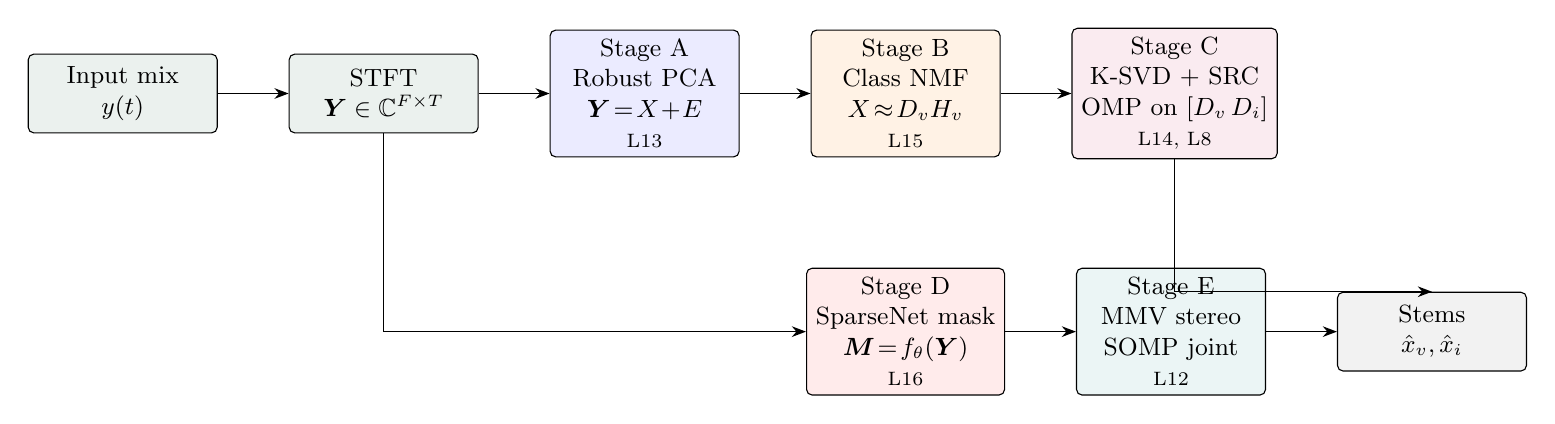
\begin{tikzpicture}[
  node distance=10mm and 9mm,
  font=\small,
  box/.style={draw, rounded corners=2pt, align=center, minimum height=10mm,
              minimum width=24mm, fill=mygreen!8, line width=0.4pt},
  rpca/.style={box, fill=blue!8},
  nmf/.style={box, fill=orange!10},
  ksvd/.style={box, fill=purple!8},
  scn/.style={box, fill=red!8},
  mmv/.style={box, fill=teal!8},
  outbox/.style={box, fill=gray!10},
  arr/.style={-{Stealth[length=1.8mm]}, line width=0.5pt}
]
\node[box] (in)   {Input mix\\$y(t)$};
\node[box, right=of in] (stft) {STFT\\$\bm{Y}\in\mathbb{C}^{F\times T}$};
\node[rpca, right=of stft]  (rpca) {Stage A\\Robust PCA\\$\bm{Y}\!=\!X\!+\!E$\\\scriptsize L13};
\node[nmf,  right=of rpca]  (nmf)  {Stage B\\Class NMF\\$X\!\approx\!D_v H_v$\\\scriptsize L15};
\node[ksvd, right=of nmf]   (ksvd) {Stage C\\K-SVD + SRC\\OMP on $[D_v\,D_i]$\\\scriptsize L14, L8};
\node[scn,  below=14mm of nmf] (scn) {Stage D\\SparseNet mask\\$\Mb\!=\!f_{\theta}(\bm{Y})$\\\scriptsize L16};
\node[mmv,  right=of scn]   (mmv)  {Stage E\\MMV stereo\\SOMP joint\\\scriptsize L12};
\node[outbox, right=of mmv] (outnode) {Stems\\$\hat{x}_v,\hat{x}_i$};

\draw[arr] (in) -- (stft);
\draw[arr] (stft) -- (rpca);
\draw[arr] (rpca) -- (nmf);
\draw[arr] (nmf) -- (ksvd);
\draw[arr] (stft.south) |- (scn.west);
\draw[arr] (scn) -- (mmv);
\draw[arr] (mmv) -- (outnode);
\draw[arr] (ksvd.south) |- (outnode.north);
\end{tikzpicture}}
\caption{The five-stage pipeline.  Each block is keyed to a specific ENGS 109
lecture.  Stages A--C are training-free classical baselines.  Stage D is
the deep-sparsity learned mask predictor that I will train on MUSDB18.
Stage E refines the result using joint sparsity across stereo channels.}
\label{fig:pipeline}
\end{figure}

\noindent
The pipeline of Figure~\ref{fig:pipeline} cascades five sparsity-aware
stages.  Each can stand alone as a separator and will be evaluated
independently before being combined.

\subsection*{Stage A. Robust PCA for harmonic--percussive split (L13)}
Apply $(P_{R_1})$ from L13~\cite{candes2011rpca}:
\[
(X^*, E^*) \;=\; \argmin_{X,\,E}\; \norm{X}_* + \lambda\,\norm{E}_1
\quad\text{s.t.}\quad \Mb_Y = X + E,
\quad \lambda = 1/\sqrt{\max(F,T)}.
\]
$X$ collects the harmonic (low-rank, sustained) content, $E$ the percussive
(sparse, transient) content.  This reproduces the Huang--Mysore--Smaragdis HPSS
baseline~\cite{hpss} and gives me my first separable two-way split for free.
I will solve $(P_{R_1})$ with the inexact-ALM solver I already wrote for PS8
(nuclear norm completion), augmented with a soft-thresholding step.

\begin{figure}[t]
\centering
\includegraphics[width=\linewidth]{figures/fig_rpca_demo.pdf}
\caption{Sanity check of my RPCA solver on a $60\!\times\!80$ synthetic
matrix with rank 3 and $5\%$ sparse corruption (magnitude up to $\pm 6$).
Inexact ALM with $\lambda{=}1/\sqrt{N_1}$ recovers the low-rank component to
within $10^{-7}$ relative Frobenius error in $32$ iterations.  The same
solver, scaled to $F\!\times\!T = 1025\!\times\!860$ spectrograms, drives
Stage~A.}
\label{fig:rpca}
\end{figure}

\subsection*{Stage B. NMF with class-conditional dictionaries (L15)}
Train two dictionaries offline on isolated stems:
\[
\D_v \;=\; \argmin_{D,H\ge 0} \norm{\Mb_{Y_v} - DH}_F^2,
\qquad
\D_i \;=\; \argmin_{D,H\ge 0} \norm{\Mb_{Y_i} - DH}_F^2,
\]
using Lee--Seung multiplicative updates with $K_v{=}K_i{=}64$ atoms.  At
test time, factorise the mixture against the concatenated dictionary
$[\D_v \mid \D_i]$ and split the activations:
\[
[H_v;\,H_i] \;=\; \argmin_{H \ge 0}\;
\norm{\Mb_Y - [\D_v\mid\D_i]\,H}_F^2
+ \beta \norm{H}_1.
\]
The vocal and instrumental magnitude reconstructions are $\D_v H_v$ and
$\D_i H_i$; soft masks come from the Wiener-style ratio
$\Mb_v = \D_v H_v / (\D_v H_v + \D_i H_i)$.  The $\beta$-divergence variant
with $\beta\!=\!1$ (Kullback--Leibler) typically beats Frobenius on audio
spectrograms~\cite{fevotte2009}; I will compare both.

\subsection*{Stage C. K-SVD discriminative dictionaries with SRC (L14, L8)}
Replace each NMF dictionary with a K-SVD-trained sparsifying dictionary
$\D_c\in\R^{F\times K_c}$ with $S$-sparse codes per spectrogram frame
$\yb\in\R^F$:
\[
\alphab^* \;=\; \argmin_{\alphab} \norm{\yb - [\D_v \mid \D_i]\alphab}_2^2
\quad\text{s.t.}\quad \norm{\alphab}_0 \le S,
\]
solved per frame by OMP (PS3).  Assign each time--frequency bin to the
class whose sub-dictionary explains it best, following the L8 residual rule
$c^* = \argmin_c \norm{\yb - \D_c \alphab^*_c}_2$.  This converts the
classical SRC face-recognition recipe into a per-bin source classifier,
which gives a binary mask that I can then soften.

\subsection*{Stage D. SparseNet mask predictor (L16)}
The headline contribution.  Replace the U-Net mask predictor used by Spleeter
and Open-Unmix~\cite{spleeter, openunmix} with a stack of Chin's composite
sparse coding modules.  Each module takes a vectorised spectrogram patch
$\xb^{(\ell)} \in \R^{N_\ell}$ and computes
\begin{align}
\alphab^{(1)} &= \argmin_{\alphab\,\ge\,0}\;
\tfrac{1}{2}\norm{\xb^{(\ell)} - \D^{(1)}\alphab}_2^2
+ \lambda_1\norm{\alphab}_1
+ \tfrac{\lambda_2}{2}\norm{\alphab}_2^2,
\label{eq:scn1}\\
\alphab^{(2)} &= \argmin_{\alphab\,\ge\,0}\;
\tfrac{1}{2}\norm{\alphab^{(1)} - \D^{(2)}\alphab}_2^2
+ \lambda_1\norm{\alphab}_1
+ \tfrac{\lambda_2}{2}\norm{\alphab}_2^2,
\label{eq:scn2}
\end{align}
where $\D^{(1)}\in\R^{N_\ell\times N_u}$ is the fat upsampling dictionary
($N_u > N_\ell$) and $\D^{(2)}\in\R^{N_u\times N_d}$ is the tall
downsampling dictionary ($N_d < N_u$).  Eq.~\eqref{eq:scn1}-\eqref{eq:scn2}
are the L16 ``composite sparse coding module'' verbatim.  Inference is run
with FISTA (L10) for 30--50 iterations; training is end-to-end backprop
through the unrolled FISTA per L16, with dictionaries $\D^{(1)},\D^{(2)}$
and shrinkage parameters $\lambda_1,\lambda_2$ as learnable parameters.

The architecture stacks $L\!=\!4$ composite modules followed by a
$1\!\times\!1$ convolution and sigmoid to emit a soft mask
$\Mb_v\in[0,1]^{F\times T}$.  Training objective:
\[
\mathcal{L}(\theta) \;=\; \norm{\Mb_v\odot\bm{Y} - \bm{Y}_v}_1
+ \mu \sum_\ell \norm{\alphab^{(\ell)}}_1,
\]
combining a magnitude-domain $\ell_1$ reconstruction loss and an explicit
sparsity penalty on every intermediate code.  $\theta = \{\D^{(\ell)},
\lambda^{(\ell)}\}$.

\subsection*{Stage E. MMV joint sparsity for stereo (L12)}
For stereo input $\bm{Y}_L,\bm{Y}_R$, stack frame-wise spectra into
$\bm{Y}=[\yb_L\;\yb_R]\in\R^{F\times 2}$ and solve the simultaneous OMP
of L12~\cite{tropp2006somp}:
\[
\bm{X}^* \;=\; \argmin_{\bm{X}}\; \norm{\bm{Y} - \D\bm{X}}_F^2
\quad\text{s.t.}\quad \norm{\bm{X}}_{\mathrm{row},0} \le S.
\]
The shared row-support enforces that the same atoms fire in both channels,
which matches the physics of a pan-mixed source.  This gives the model a
stereo prior for free that Spleeter/Open-Unmix do not encode explicitly.

% ====================================================================
\section{Connection to ENGS 109 material}
Table~\ref{tab:map} traces every method block back to a specific lecture and
to code I have already written for the problem sets.

\begin{table}[h]
\small
\centering
\caption{Each stage maps to a course lecture and reuses problem-set code.}
\label{tab:map}
\begin{tabular}{@{}llll@{}}
\toprule
\textbf{Stage} & \textbf{Mathematical object} & \textbf{Lecture} &
\textbf{PS code reused} \\
\midrule
A. Robust PCA      & $\min\,\norm{X}_* + \lambda\norm{E}_1$
                   & L13 Matrix Completion
                   & PS8 (nuclear-norm SVT) \\
B. NMF             & $Y\!\approx\!DH,\;D,H\!\ge\!0$
                   & L15 NMF
                   & New module (sklearn baseline) \\
C. K-SVD + SRC     & $\min\norm{\alpha}_0,\;Y\!=\!D\alpha$
                   & L14 Dict.\ Learning, L8 SRC
                   & PS3 (OMP), PS7 (SRC) \\
D. SparseNet       & Stacked Eqs.~\eqref{eq:scn1}-\eqref{eq:scn2}
                   & L16 Deep Sparsity
                   & PS5 (FISTA), PS7 (Lasso) \\
E. MMV / SOMP      & $\min\,\norm{X}_{1,2},\;Y\!=\!DX$
                   & L12 Multi-Measurement
                   & PS3 (OMP) extended \\
\bottomrule
\end{tabular}
\end{table}

Every theoretical guarantee we proved in class has a direct consequence
in the proposal:
\begin{itemize}
\item RIP with $\delta_{2S}<\sqrt{2}-1$ (L6, Cand\`es) bounds the
recovery error of the NMF/K-SVD activation estimates from
Stage B and C.  For the over-complete dictionaries I plan to learn,
$M$ corresponds to the number of frequency bins ($F\!=\!1025$ at
$N_{\text{FFT}}{=}2048$) and $N$ to the number of dictionary atoms
($K\!=\!64$ per source), giving $M{\gg}N$ and easy RIP satisfaction.
\item Cand\`es--Recht (L13, Thm.~1) gives $|\Omega|\ge CN^{5/4} r\log N$
for matrix completion; with $F\!=\!1025$, $T\!\approx\!860$ for a 20-s clip,
and assumed harmonic rank $r\!=\!8$, the implied $|\Omega|$ is well within
the $\approx 88\%$ of bins we observe (the $12\%$ unobserved are the
percussive sparse part).
\item Robust PCA (L13, Thm.~2) sets $\lambda{=}1/\sqrt{N_1}$ canonically.
That single hyper-parameter choice removes most of the manual tuning that
HPSS papers~\cite{hpss} have historically wrestled with.
\item SparseNet's L16 result: $83.11\%$ on STL-10 vs $76.29\%$ for a
matched CNN.  That experiment used $5{,}000$ labelled images, the same
order of magnitude as MUSDB18-HQ's $100$ training songs.  The hypothesis
that motivates Stage D is that the same data-efficiency win transfers
to spectrogram-domain regression.
\end{itemize}

% ====================================================================
\section{Evaluation plan}
\paragraph{Dataset.} MUSDB18-HQ~\cite{musdb18hq}, the standard music
source-separation benchmark: $100$ training songs and $50$ test songs at
$44.1$~kHz with fully isolated vocals/drums/bass/other stems.

\paragraph{Metrics.} Median test-set SDR, SI-SDR, SIR, SAR via
\texttt{mir\_eval}~\cite{mireval} and \texttt{museval}~\cite{museval}, each
broken out per stem.  Vocals SDR is the headline number reported in
SiSEC~\cite{sisec18}.

\paragraph{Baselines.} I will compare against
(i) ElevenLabs voice isolation (my thesis baseline),
(ii) REPET-SIM~\cite{repetsim} (classical similarity-matrix baseline),
(iii) Spleeter pre-trained 2-stem~\cite{spleeter},
(iv) Open-Unmix UMX-L pre-trained~\cite{openunmix}, and
(v) Demucs v4 pre-trained~\cite{demucs}.

\paragraph{Targeted improvement.} Match Spleeter ($\approx 6.5$~dB vocal
SDR on MUSDB18 test) with Stages A--C alone; reach within $2$~dB of
Demucs v4 ($\approx 8.5$~dB) with Stage D.

\paragraph{Listening study.} Eight Mozart~AI beta users grade $20$
randomly chosen $10$-s test clips on a $5$-point MUSHRA-like scale.
This addresses the well-known SDR/perceived-quality
mismatch~\cite{cano2019}.

% ====================================================================
\section{Timeline (10-week solo schedule)}
\noindent\begin{tabular}{@{}llp{0.66\linewidth}@{}}
\textbf{Weeks 1--2.}  &  Data + baselines & MUSDB18-HQ loader; STFT/CQT
                                            pipeline; Stage A (RPCA),
                                            Stage B (NMF) working
                                            end-to-end.\\
\textbf{Weeks 3--4.}  &  Classical stack  & Stage C (K-SVD + SRC); ablation
                                            of $K, S$; metric harness;
                                            first set of qualitative figures.\\
\textbf{Weeks 5--6.}  &  SparseNet build  & Stage D unrolled FISTA;
                                            backward pass verification on a
                                            toy denoising task; first
                                            spectrogram-mask training.\\
\textbf{Weeks 7--8.}  &  Full training    & MUSDB18 training of Stage D
                                            on Discovery cluster GPUs;
                                            Stage E stereo refinement.\\
\textbf{Weeks 9--10.} &  Write-up         & Final report, figures, listening
                                            study, code release on my
                                            GitHub.
\end{tabular}

% ====================================================================
\section{Risks and mitigations}
\begin{itemize}
\item \textbf{SparseNet training cost.}  L16 itself notes ``take much longer
training time.''  Mitigation: cap Stage D at $L\!=\!4$ composite modules,
use mel-band spectrograms ($64$ bins) instead of full STFT to keep
$N_\ell$ small, and budget one GPU-week.  Fallback: ship Stages A--C +
a small UNet-style mask CNN as Stage D'.
\item \textbf{NMF convergence on full-resolution spectrograms.}
$1025\!\times\!860\!\times\!100$ songs is a lot of data for multiplicative
updates.  Mitigation: subsample frames; use Online NMF~\cite{onlinenmf}.
\item \textbf{Phase reconstruction.}  Magnitude masking + mixture phase is
known to introduce artefacts.  Mitigation: report metrics with and without
Griffin--Lim phase refinement; cite as a limitation rather than try to
fix it inside a 10-week scope.
\item \textbf{Dataset license.}  MUSDB18-HQ is research-only; no plan to
ship trained weights commercially.  All MUSDB-derived audio stays
inside the report.
\end{itemize}

% ====================================================================
\section{Deliverables}
A self-contained GitHub repository,
\texttt{takakhoo/engs109-music-separation}, with:
(1) the LaTeX final report including ablations and listening-study
results; (2) reproducible \texttt{train.py}/\texttt{evaluate.py} entry
points; (3) Jupyter notebooks for each stage A--E mirroring the PS
format; (4) audio examples and pre-computed spectrograms for the
report figures; (5) the trained Stage D checkpoint (under MUSDB
license terms).

% ====================================================================
{\small
\begin{thebibliography}{99}
\bibitem{mireval} C.\ Raffel \emph{et al.},
``mir\_eval: A transparent implementation of common MIR metrics,''
\textit{ISMIR}, 2014.

\bibitem{demucs} A.\ D\'efossez,
``Hybrid spectrogram and waveform source separation,''
\textit{MDX Workshop @ ISMIR}, 2021.

\bibitem{lerouxsdr} J.\ Le~Roux \emph{et al.},
``SDR -- half-baked or well done?,''
\textit{ICASSP}, 2019.

\bibitem{candes2009} E.\ J.\ Cand\`es and B.\ Recht,
``Exact matrix completion via convex optimization,''
\textit{Found.\ Comput.\ Math.}, vol.~9, pp.~717--772, 2009.

\bibitem{candes2011rpca} E.\ J.\ Cand\`es, X.\ Li, Y.\ Ma, and J.\ Wright,
``Robust principal component analysis?,''
\textit{Journal of the ACM}, vol.~58, no.~3, 2011.

\bibitem{hpss} P.-S.\ Huang, S.\ D.\ Chen, P.\ Smaragdis, and M.\ Hasegawa-Johnson,
``Singing-voice separation from monaural recordings using robust principal
component analysis,'' \textit{ICASSP}, 2012.

\bibitem{fevotte2009} C.\ F\'evotte, N.\ Bertin, and J.-L.\ Durrieu,
``Nonnegative matrix factorization with the Itakura--Saito divergence,''
\textit{Neural Computation}, vol.~21, pp.~793--830, 2009.

\bibitem{tropp2006somp} J.\ A.\ Tropp,
``Algorithms for simultaneous sparse approximation. Part I: greedy pursuit,''
\textit{Signal Processing}, vol.~86, pp.~572--588, 2006.

\bibitem{spleeter} R.\ Hennequin \emph{et al.},
``Spleeter: a fast and efficient music source separation tool,''
\textit{Journal of Open Source Software}, vol.~5, 2020.

\bibitem{openunmix} F.-R.\ St\"oter \emph{et al.},
``Open-Unmix: A reference implementation for music source separation,''
\textit{JOSS}, 2019.

\bibitem{musdb18hq} Z.\ Rafii \emph{et al.},
``MUSDB18-HQ: an uncompressed version of MUSDB18,''
\textit{Zenodo}, 2019.

\bibitem{museval} F.-R.\ St\"oter, A.\ Liutkus, and N.\ Ito,
``The 2018 Signal Separation Evaluation Campaign,''
\textit{LVA/ICA}, 2018.

\bibitem{sisec18} F.-R.\ St\"oter \emph{et al.},
``SiSEC 2018,'' \textit{ICA}, 2018.

\bibitem{repetsim} Z.\ Rafii and B.\ Pardo,
``Music/voice separation using the similarity matrix,''
\textit{ISMIR}, 2012.

\bibitem{cano2019} E.\ Cano \emph{et al.},
``Musical source separation: an introduction,''
\textit{IEEE Signal Processing Magazine}, vol.~36, no.~1, 2019.

\bibitem{onlinenmf} A.\ Lefevre, F.\ Bach, and C.\ F\'evotte,
``Online algorithms for nonnegative matrix factorization with the
Itakura--Saito divergence,'' \textit{WASPAA}, 2011.

\bibitem{sun2018scn} X.\ Sun, N.\ M.\ Nasrabadi, and T.\ D.\ Tran,
``Supervised multilayer sparse coding networks for image
classification,'' arXiv:1701.08349 (cited in L16), 2017.

\bibitem{khoo2025tokenunet} T.\ Khoo,
``Token U-Net: Neural Audio Codec Remastering for Full-Mix Music
Restoration,'' Honors Thesis, Dartmouth College, Peter Chin
(primary advisor), 2025.

\bibitem{encodec} A.\ D\'efossez, J.\ Copet, G.\ Synnaeve, and Y.\ Adi,
``High fidelity neural audio compression (EnCodec),''
\textit{Transactions on Machine Learning Research}, 2023.

\bibitem{smaragdis2007nmf} P.\ Smaragdis,
``Convolutive speech bases and their application to supervised speech
separation,'' \textit{IEEE TASLP}, vol.\ 15, no.\ 1, 2007.

\bibitem{aharon2006ksvd} M.\ Aharon, M.\ Elad, and A.\ Bruckstein,
``K-SVD: an algorithm for designing overcomplete dictionaries for
sparse representation,'' \textit{IEEE TSP}, vol.\ 54, no.\ 11, 2006.

\bibitem{gregor2010lista} K.\ Gregor and Y.\ LeCun,
``Learning fast approximations of sparse coding,''
\textit{ICML}, 2010.
\end{thebibliography}
}

\end{document}
